\newif\ifelsevierclass
\IfFileExists{elsarticle.cls}{%
  \elsevierclasstrue\documentclass[preprint,12pt]{elsarticle}%
}{%
  \elsevierclassfalse\documentclass[11pt]{article}%
}

\usepackage[T1]{fontenc}
\usepackage[utf8]{inputenc}
\usepackage{lmodern}
\usepackage{microtype}
\usepackage{amsmath,amssymb}
\usepackage{booktabs}
\usepackage{longtable}
\usepackage{array}
\usepackage{graphicx}
\graphicspath{{figures/}{./}}
\usepackage{xcolor}
\usepackage{enumitem}
\usepackage{threeparttable}
\usepackage{tabularx}
\usepackage{etoolbox}
\usepackage{tikz}
\usetikzlibrary{arrows.meta}
\ifelsevierclass\else
  \usepackage[margin=1in]{geometry}
  \usepackage[numbers,sort&compress]{natbib}
\fi
\usepackage{xurl}
\usepackage[hidelinks,breaklinks=true]{hyperref}
\usepackage[nameinlink,noabbrev]{cleveref}
\urlstyle{same}
\Urlmuskip=0mu plus 1mu\relax

\AtBeginEnvironment{thebibliography}{%
  \setlength{\emergencystretch}{2em}%
}

\setlist{nosep,leftmargin=*}
\renewcommand{\arraystretch}{1.15}
\ifelsevierclass
  \biboptions{numbers,sort&compress}
\fi
\newcommand{\rx}[1]{\texttt{\detokenize{#1}}}

\newcommand{\insightbox}[2]{%
  \begin{center}
  \setlength{\fboxsep}{6pt}%
  \fcolorbox{black!25}{black!3}{%
    \parbox{0.88\linewidth}{%
      \small\textbf{#1} #2%
    }%
  }%
  \end{center}
}

\newcommand{\papertitle}{Threat Attention and Limited Preparedness Attention Following AI Extinction Warnings}

\newcommand{\abstracttext}{
Catastrophic artificial-intelligence (AI) warnings often identify critical infrastructure as a pathway through which severe harm could propagate. Yet drawing attention to a threat is not the same as directing attention toward the capacity to withstand or control it. We examine this distinction across two prominent AI extinction-warning episodes: the May 2023 Statement on AI Risk and a September 2026 warning episode. Using English Wikipedia pageviews, targeted news framing, and prespecified equity portfolios, we measure how attention was distributed between catastrophic consequences and protective capacity.

We operationalize a \emph{threat--preparedness gap} (TPG) as the difference between abnormal information seeking about existential consequences and attention to safety/governance, infrastructure/resilience, and shutdown/control. The imbalance was substantially larger in 2026. Existential-threat attention reached 41.3 standardized-deviation days (SD-days), compared with 3.7 for infrastructure/resilience and 7.0 for shutdown/control. The mean daily TPG increased from 2.97 in 2023 to 7.96 in 2026, a 2.7-fold difference.

The surrounding information environment showed a similar asymmetry: existential media framing was positively associated with existential-threat attention in both episodes, whereas infrastructure framing was not associated with infrastructure/resilience attention. Equity markets displayed a different response. Across the 2026 episode window and every prespecified post-event window, the cybersecurity/resilience portfolio outperformed its modeled benchmark by 11.3\% to 13.6\%, compared with $-1.6\%$ to $+1.3\%$ for AI-infrastructure firms.

These findings show that catastrophic AI warnings can generate intense attention to the threat without a proportional shift toward preparedness. For critical infrastructure protection, the distinction matters because making a threat salient is not the same as making protective capacity salient. Public information seeking and market repricing also need not point in the same direction, underscoring the value of measuring these response channels separately.
}

\ifelsevierclass
  \journal{International Journal of Critical Infrastructure Protection}
\fi

\begin{document}
\ifelsevierclass
\begin{frontmatter}

\title{\papertitle}

\author[uccs,usafa]{Bonnie Rushing}
\author[uccs,usafa]{Ethan Anderson}
\author[uccs]{Shouhuai Xu}
\affiliation[uccs]{organization={University of Colorado Colorado Springs},
  city={Colorado Springs},
  state={Colorado},
  country={United States}}
\affiliation[usafa]{organization={US Air Force Academy},
  city={Colorado Springs},
  state={Colorado},
  country={United States}}

\begin{abstract}
\abstracttext
\end{abstract}

\begin{keyword}
critical infrastructure protection \sep artificial intelligence \sep resilience \sep information seeking \sep risk communication \sep event study
\end{keyword}

\end{frontmatter}
\else
\title{\papertitle}
\author{%
  Bonnie Rushing\\
  {\small University of Colorado Colorado Springs}\\
  {\small US Air Force Academy}
  \and
  Ethan Anderson\\
  {\small University of Colorado Colorado Springs}\\
  {\small US Air Force Academy}
  \and
  Shouhuai Xu\\
  {\small University of Colorado Colorado Springs}%
}
\date{\today}
\maketitle
\begin{abstract}
\abstracttext
\end{abstract}
\noindent\textbf{Keywords:} critical infrastructure protection; artificial intelligence; resilience; information seeking; risk communication; event study
\fi

\section{Introduction}

Public warnings about artificial intelligence increasingly combine extraordinary severity with substantial uncertainty. In May 2023, hundreds of researchers and technology leaders endorsed a statement declaring that mitigating AI extinction risk should be treated as a global priority alongside pandemics and nuclear war \citep{cais2023statement}. Surveys of AI researchers document wide disagreement about timelines while recording nontrivial concern about outcomes as severe as human extinction \citep{grace2025thousands}.

For critical infrastructure protection (CIP), the analytically relevant feature of these warnings is not their severity alone, but the mechanism through which harm could propagate. Catastrophic AI scenarios are routinely described as operating through networked and critical systems, including digital infrastructure, energy grids, financial systems, healthcare, transportation, and biological or chemical pathways \citep{bengio2026aisafety}.
If a warning raises the salience of those pathways, one would expect attention to move toward the systems at risk, and toward mechanisms that could interrupt or absorb a failure: resilience, continuity, incident response, capability control, and emergency shutdown \citep{bengio2026aisafety,orseau2016interruptible}. If, instead, attention stops at the abstract end state, then a warning that names infrastructure as the pathway is not, in practice, producing an infrastructure-oriented response.

The distinction became observable in September 2026. On September 8, Anthropic researcher, Jacob Coxon, announced his resignation and argued that frontier laboratories were moving irresponsibly toward self-improving superintelligence. Mainstream coverage began on September 9 \citep{bellan2026gambling}; other researchers amplified the warning, and U.S. lawmakers publicly called for additional oversight \citep{rozen2026lawmakers}. 
By September 14, AI-linked stocks were under pressure after prominent executives cited safety risks and called for slower development \citep{reuters2026markets}. Rather than a single instantaneous shock, these events form a short, traceable warning episode with channel-specific amplification dates.

This paper asks how collective attention changes during such an episode and, in particular, how much attention reaches protective capacity. We examine two aggregate behavioral responses: Wikipedia pageviews for preregistered information families and equity repricing in prespecified stock portfolios. We also analyze news framing to test whether infrastructure-oriented coverage corresponds with subsequent infrastructure-oriented attention.

The study makes three contributions to CIP research. 
First, it operationalizes the \emph{threat--preparedness gap} as a behavioral attention measure: the difference between abnormal information seeking about catastrophic consequences and abnormal information seeking about protective capacity.
Second, it distinguishes infrastructure resilience from broader AI safety/governance and from specific control mechanisms such as emergency shutdown. 
Third, it identifies a cross-channel difference: infrastructure/resilience drew relatively little Wikipedia attention, but the largest equity-market response among the portfolios studied.

Prior work has identified threat--preparedness gaps in perceived societal readiness for other hazards \citep{howarth2025heat} and has distinguished societal threat from efficacy in AI risk communication \citep{schwarz2024rage,schwarz2024mediated}. We extend this distinction to observed information-seeking behavior, asking whether attention elicited by an AI risk warning moves toward protective capacity as well as toward the threat itself.

We emphasize at the outset what these measures cannot do. Pageviews are aggregate counts, not counts of unique people; they do not reveal why a page was opened or whether anyone acted afterward. Nothing here identifies panic, fear, efficacy, or offline preparation. The claims are about the observable direction of collective attention, and are bounded accordingly.


\section{Conceptual Background}

Related research has examined several components of this problem separately. Studies of AI risk communication distinguish societal threat from societal efficacy and show that AI narratives vary substantially in the extent to which they emphasize risks and corresponding risk-control measures \citep{schwarz2024rage,schwarz2024mediated}. Separately, studies of health crises demonstrate that Wikipedia pageviews provide a behavioral trace of collective information seeking and can closely correspond with news exposure \citep{tizzoni2020zika,gozzi2020covid}. Recent work also cautions that equating AI safety primarily with existential risk can obscure a broader range of concrete safety concerns \citep{gyevnar2025safety}. Building on these literatures, we examine not simply whether an AI warning attracts attention, but how that attention is allocated between catastrophic consequences and protective capacity. We operationalize this allocation as a behavioral threat--preparedness gap and examine it alongside media framing and equity repricing. 


\subsection{Risk warnings and information seeking}

Risk communication research treats information seeking as a response shaped by perceived hazard, affect, knowledge insufficiency, social expectations, and beliefs about the usefulness and accessibility of information channels \citep{griffin1999risp,kahlor2010prism}. 
Meta-analytic evidence broadly supports the Risk Information Seeking and Processing model while showing that its components differ in explanatory power \citep{yang2014meta}. A dramatic warning can create a perceived gap between what an audience knows and what it believes it needs to know. That does not imply that the resulting search is oriented toward protective action.

The Extended Parallel Process Model distinguishes responses centered on controlling a danger from responses centered on managing fear \citep{witte1992eppm}. High perceived threat combined with efficacy can motivate protective action; high threat without efficacy can produce defensive or non-protective responses.

Catastrophic AI is a plausible candidate for a gap between threat attention and preparedness attention. It has characteristics associated with ``dread'' risks: potentially catastrophic consequences, involuntariness, unfamiliarity, and uncertainty \citep{slovic1987risk}. At the same time, the protective actions available to an ordinary individual are unclear, and the actions available to infrastructure operators are not the subject of general audience coverage.


\subsection{Wikipedia pageviews as behavioral traces}

Researchers have used Wikipedia activity to measure rapid changes in collective attention during crises \citep{palen2016crisis,ribeiro2021wikipedia}. Temporal patterns also distinguish brief spikes from persistent or renewed attention \citep{rushing2026thee}, which is important when comparing threat-oriented and preparedness-oriented responses.

Pageviews do not reveal why a page was opened, whether it was read carefully, or how the reader interpreted it. Nevertheless, they do provide an aggregate behavioral trace of information access \citep{dimitrov2018query}. We therefore refer to information seeking measured through Wikipedia pageviews, not ``searches.''


\subsection{Critical-infrastructure protection as an information response}

Protection depends not only on technical controls but on whether operators, policymakers, firms, and the broader public recognize plausible failure mechanisms and direct attention toward resilience. CIP research emphasizes human judgment in risk assessment \citep{papamichael2024risk} and situation awareness in cyber resilience \citep{bellini2025situation}. Extinction warnings frequently cite infrastructure pathways, yet mainstream attention may remain fixed on the abstract end state.

Thus, we treat infrastructure-oriented information seeking as a substantive outcome and decompose it. Attention to \emph{systems that could be disrupted} (e.g., critical infrastructure, cyber--physical systems), to \emph{protective processes} (e.g., resilience, incident response, continuity, disaster recovery), and to \emph{control interventions} (e.g., kill switch, capability control, fail-safe, shutdown) are conceptually distinct. 
Searching for a kill switch reflects interest in a concrete interruption mechanism; searching for critical infrastructure reflects attention to the protected system. Neither demonstrates that anyone took protective action.

The kill-switch concept was politically salient before the September episode. U.S. lawmakers proposed an AI Kill Switch Act in July 2026, and OpenAI discussed automated shutdown capabilities in early September \citep{rozen2026killswitch,reuters2026shutdown}. We model those dates explicitly, report the kill-switch series separately, and test whether the September episode produced attention beyond the pre-existing trend.


\subsection{Media frames as the information environment}

A media ``frame'' emphasizes a particular interpretation of an event, such as its cause, consequences, or appropriate response \citep{entman1993framing}. AI extinction warnings may therefore be framed around loss of control, infrastructure compromise, biological misuse, economic disruption, governance, technical capability, or skepticism. These frames make different aspects of the same warning salient.

We use daily frame prevalence to characterize the retrieved information environment. Frame prevalence describes which interpretations were available, not whether readers noticed or accepted them.

This distinction is especially important for critical infrastructure protection. Media coverage may increase the salience of an issue without determining where public attention subsequently moves. Readers encountering a concrete account of cyber or infrastructure compromise may seek information about resilience and protection, or they may redirect their attention toward the more abstract and sensational prospect of human extinction. 
We test this correspondence by comparing the prevalence of each media frame on day $t$ with abnormal attention to the theoretically corresponding Wikipedia family from day $t$ through day $t+3$. A matching response indicates that public information seeking followed the mechanism emphasized in coverage; a mismatch indicates that attention shifted to another aspect of the warning. Because media coverage and information seeking may both respond to the same underlying event, this temporal correspondence is not interpreted as proof of individual exposure, frame acceptance, or causal persuasion.


\subsection{Financial repricing as a second revealed response}

Event studies estimate whether security returns around a dated event differ from returns predicted by a market model \citep{mackinlay1997event}. Equity markets provide a second aggregate response channel drawn from a population different from Wikipedia readers. If market participants expect an AI-risk episode to affect demand for safeguards, cybersecurity and resilience firms may be repriced differently from firms more directly exposed to AI capability development. Comparing the channels is informative precisely because they measure different behaviors in different populations.

The financial analysis is more cautious than the attention analysis. Anthropic and OpenAI were not publicly traded, other information arrives in the same window, and firm-specific announcements can dominate a short window. We address these directly in \cref{sec:robust}.


\section{Research Questions}

This paper aims to answer the following Research Questions (RQs):

\begin{description}%[style=nextline]
  \item[RQ1 --- Magnitude.] Is a high-profile AI extinction warning followed by abnormal information seeking? (Measured as standardized abnormal English Wikipedia attention over \( [0,+3] \) days.)
\item[RQ2 --- Direction.] How is abnormal attention distributed across the six information families, and does infrastructure/resilience or shutdown/control attention exceed its placebo range?
\item[RQ3 --- The threat--preparedness gap.] How large is the contrast between threat-oriented and preparedness-oriented attention, and does it differ between the May 2023 statement and the September 2026 episode?
\item[RQ4 --- Frame--attention correspondence.] Does daily media framing correspond with same-day or subsequent attention to the matching Wikipedia family, particularly for infrastructure, control, and existential threat?
\item[RQ5 --- Market divergence.] Do AI-exposed and cybersecurity/resilience stock portfolios earn different cumulative abnormal returns over the 2026 episode, and how does that compare with the public attention response?
\end{description}


\section{Research Design}

To orient the reader, Figure \ref{fig:roadmap} summarizes the study design: two warning episodes are analyzed using three data streams, which are then used to estimate abnormal attention, the threat--preparedness gap, frame--attention correspondence, and market repricing. To limit outcome-driven analytical choices, we specified event definitions, Wikipedia page families, portfolio membership, and primary analysis windows before examining the corresponding post-event outcomes.

\begin{figure}[ht!]
\centering
\scriptsize
\fbox{
\parbox{0.99\linewidth}{
\centering
\textbf{AI warning episodes}
(May 2023; Sept.\ 2026)
\; $\rightarrow$ \;\\
\textbf{Data streams}
(Wikipedia pageviews; news headlines; equity prices)
\; $\rightarrow$ \;\\
\textbf{Analyses}
(abnormal attention; TPG; frame--attention correspondence; abnormal returns)
\; $\rightarrow$ \;\\
\textbf{Inference}
(compare threat attention, preparedness attention, framing, and market repricing)
}}
\caption{Overview of the research design.}
\label{fig:roadmap}
\end{figure}


\subsection{Case selection and event timing}

The primary case is the September 2026 warning episode. The replication case is the May 30, 2023 Statement on AI Risk (\cref{tab:events}). The replication does not assume the two messages are equivalent; it tests whether the measurement framework recovers comparable or changing response profiles across two prominent warnings separated by more than three years.

\begin{table}[ht!]
\centering
\small
\caption{Prespecified events and channel-specific time zero}
\label{tab:events}
\begin{threeparttable}
\begin{tabular}{@{}>{\raggedright\arraybackslash}p{0.21\linewidth}>{\raggedright\arraybackslash}p{0.3\linewidth}>{\raggedright\arraybackslash}p{0.43\linewidth}@{}}
\toprule
Date & Analytical role & Definition \\
\midrule
30 May 2023 & Replication event, $t_0$ & Public release of the Statement on AI Risk \citep{cais2023statement}. \\
8--9 Sep 2026 & Primary attention event, $t_0$ = 9 Sep & Researcher announcement on 8 Sep; first major coverage \& broad public availability on 9 Sep \citep{bellan2026gambling}. \\
10--13 Sep 2026 & Amplification interval & Additional expert, policy, \& executive reactions; analyzed as part of the episode, not as statistically independent shocks \citep{rozen2026lawmakers}. \\
14 Sep 2026 & Primary market event, $t_0$ & First U.S. session after the executive slowdown calls became a dominant financial story \citep{reuters2026markets}.\\
\bottomrule
\end{tabular}
\begin{tablenotes}[flushleft]\footnotesize
\item Event dates, and the placement of each event's Wikipedia baseline (\cref{sec:windows}), are in \texttt{config/events.yml}.
\end{tablenotes}
\end{threeparttable}
\end{table}


\subsection{Observation windows}
\label{sec:windows}

The Wikipedia analysis uses a 56-day baseline that covers eight full weeks, allowing the model to account for normal day-of-week differences. For the 2023 statement, the baseline is $[-56,-1]$. For 2026, it is $[-57,-2]$ because the warning began on 8 September, one day before the 9 September attention event; including 8 September would contaminate the baseline and condition the AR(1) forecast on an event-related observation.

\Cref{fig:observation-windows} summarizes the event dates and every window used below. \Cref{sec:measures} defines the estimators that use them. The primary outcome is cumulative abnormal attention over $[0,+3]$. The longer prespecified $[0,+7]$ and $[0,+14]$ windows are also fully observed for both episodes as of the 27 September 2026 data cutoff, and we report all three. We retain $[0,+3]$ as the primary window for two reasons. It is the window the preregistration names first, and the negative-control pages show that counterfactual drift accumulates with window length in the 2023 episode (\cref{sec:robust}), so the shorter window is the one least dependent on the drift adjustment.

For equities, the market model is estimated over trading days $[-250,-30]$ relative to the market event date. Ending the estimation period 30 trading days before the event creates a buffer that reduces the likelihood that warning-related information influences the model used to calculate expected returns. Because the September 2026 warning developed through a sequence of announcements and reactions rather than a single disclosure, we additionally report cumulative abnormal returns across all trading sessions falling between September 8 and September 14. This episode-level window captures the market's response to the accumulating information while distinguishing it from the conventional single-day event estimate.

\begin{figure}[t]
\centering
\resizebox{\linewidth}{!}{%
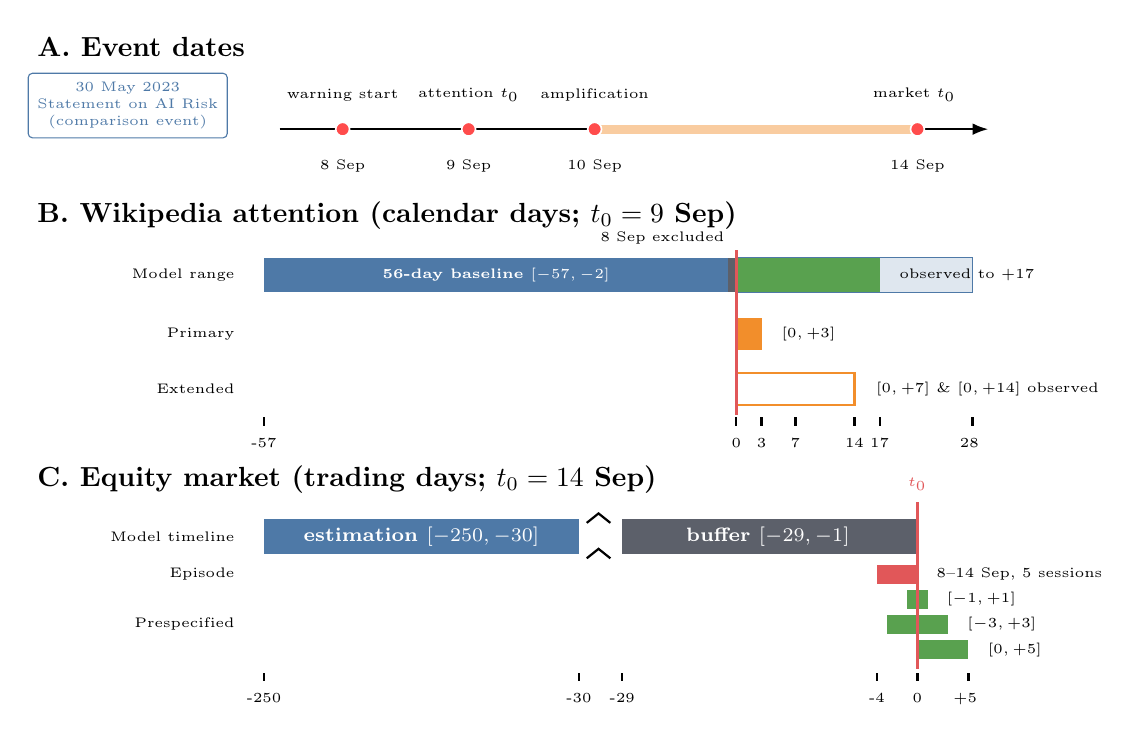
\begin{tikzpicture}[
  font=\tiny,
  axis/.style={draw=black, line width=0.8pt},
  event/.style={
    circle,
    fill=red!70,
    draw=white,
    line width=0.6pt,
    minimum size=5pt,
    inner sep=0pt
  },
  note/.style={font=\tiny, align=center}
]

% Colors
\definecolor{windowblue}{HTML}{4E79A7}
\definecolor{windowgreen}{HTML}{59A14F}
\definecolor{windoworange}{HTML}{F28E2B}
\definecolor{windowred}{HTML}{E15759}
\definecolor{windowgray}{HTML}{5C606A}

% ------------------------------------------------------------
% A. Event dates
% ------------------------------------------------------------
\node[anchor=west,font=\bfseries] at (0,6.4)
  {A. Event dates};

\node[
  draw=windowblue,
  rounded corners=1.5pt,
  text=windowblue,
  font=\tiny,
  align=center,
  anchor=west
] at (0,5.65)
  {30 May 2023\\
   Statement on AI Risk\\
   (comparison event)};

\draw[axis,-{Latex[length=2mm]}] (3.2,5.35)--(12.2,5.35);
\draw[line width=3.2pt,windoworange!45]
  (7.2,5.35)--(11.3,5.35);

\foreach \x/\date/\lab in {
  4.0/{8 Sep}/{warning start},
  5.6/{9 Sep}/{attention $t_0$},
  7.2/{10 Sep}/{amplification},
  11.3/{14 Sep}/{market $t_0$}
}{
  \node[event] at (\x,5.35) {};
  \node[note,anchor=north] at (\x,5.08) {\date};
  \node[note,anchor=south] at (\x,5.58) {\lab};
}

% ------------------------------------------------------------
% B. Wikipedia windows
% ------------------------------------------------------------
\node[anchor=west,font=\bfseries] at (0,4.25)
  {B. Wikipedia attention
   (calendar days; $t_0=9$ Sep)};

\node[anchor=east] at (2.75,3.50) {Model range};

\fill[windowblue]
  (3.0,3.28) rectangle (8.89,3.72);

\node[text=white,font=\bfseries\tiny] at (5.95,3.50)
  {56-day baseline $[-57,-2]$};

% 8 Sep (day -1): warning begins; excluded from the baseline, scored out of
% sample.
\fill[windowgray]
  (8.89,3.28) rectangle (9.0,3.72);
\node[note,anchor=south east] at (8.97,3.76)
  {8 Sep excluded};

\fill[windowblue!18]
  (9.0,3.28) rectangle (12.0,3.72);

\draw[windowblue]
  (9.0,3.28) rectangle (12.0,3.72);

\fill[windowgreen]
  (9.0,3.28) rectangle (10.82,3.72);

\node[note,anchor=west] at (10.95,3.50)
  {observed to $+17$};

\node[anchor=east] at (2.75,2.75) {Primary};

\fill[windoworange]
  (9.0,2.55) rectangle (9.32,2.95);

\node[note,anchor=west,font=\tiny\bfseries]
  at (9.45,2.75) {$[0,+3]$};

\node[anchor=east] at (2.75,2.05) {Extended};

\draw[
  windoworange,
  line width=0.8pt
] (9.0,1.85) rectangle (10.50,2.25);

\node[note,anchor=west] at (10.65,2.05)
  {$[0,+7]$ \& $[0,+14]$ observed};

\draw[windowred,line width=0.9pt]
  (9.0,1.72)--(9.0,3.82);

\foreach \x/\lab in {
  3/{-57},
  9/{0},
  9.32/{3},
  9.75/{7},
  10.5/{14},
  10.82/{17},
  12/{28}
}{
  \draw[axis] (\x,1.69)--(\x,1.58);
  \node[note,anchor=north] at (\x,1.55) {\lab};
}

% ------------------------------------------------------------
% C. Equity-market windows
% ------------------------------------------------------------
\node[anchor=west,font=\bfseries] at (0,0.90)
  {C. Equity market
   (trading days; $t_0=14$ Sep)};

\node[anchor=east] at (2.75,0.18) {Model timeline};

\fill[windowblue]
  (3.0,-0.05) rectangle (7.0,0.40);

\node[text=white,font=\bfseries\scriptsize] at (5.0,0.18)
  {estimation $[-250,-30]$};

\draw[axis] (7.10,-0.10)--(7.25,0.02)--(7.40,-0.10);
\draw[axis] (7.10,0.35)--(7.25,0.47)--(7.40,0.35);

\fill[windowgray]
  (7.55,-0.05) rectangle (11.30,0.40);

\node[text=white,font=\bfseries\scriptsize] at (9.40,0.18)
  {buffer $[-29,-1]$};

\node[anchor=east] at (2.75,-0.30) {Episode};

\fill[windowred]
  (10.783,-0.42) rectangle (11.30,-0.18);

\node[note,anchor=west] at (11.42,-0.30)
  {8--14 Sep, 5 sessions};

\node[anchor=east] at (2.75,-0.94) {Prespecified};

\fill[windowgreen]
  (11.171,-0.74) rectangle (11.429,-0.50);

\node[note,anchor=west] at (11.55,-0.62) {$[-1,+1]$};

\fill[windowgreen]
  (10.912,-1.06) rectangle (11.688,-0.82);

\node[note,anchor=west] at (11.81,-0.94) {$[-3,+3]$};

\fill[windowgreen]
  (11.30,-1.38) rectangle (11.947,-1.14);

\node[note,anchor=west] at (12.07,-1.26) {$[0,+5]$};

\draw[windowred,line width=0.9pt]
  (11.30,-1.50)--(11.30,0.62);

\node[note,text=windowred,anchor=south]
  at (11.30,0.64) {$t_0$};

\foreach \x/\lab in {
  3/{-250},
  7/{-30},
  7.55/{-29},
  10.783/{-4},
  11.3/{0},
  11.947/{+5}
}{
  \draw[axis] (\x,-1.56)--(\x,-1.66);
  \node[note,anchor=north] at (\x,-1.69) {\lab};
}
\end{tikzpicture}%
}
\caption{\textbf{Event dates and observation windows.} Solid bars denote observed periods. At the 27 September 2026 data cutoff the pageviews API had published through 26 September ($t_0+17$) and the last trading session was 25 September, so every prespecified window in panels B and C is fully observed; the extended attention windows are drawn solid because they now fall inside the published range. Panel C shows the three prespecified market windows in green alongside the episode window; all four are measured in trading days from the market $t_0$ of 14 September. The 2026 Wikipedia baseline ends on 7 September so that 8 September, when the warning began, is not used to estimate normal attention.}
\label{fig:observation-windows}
\end{figure}



\section{Data}
\subsection{Wikipedia information seeking}

We retrieve daily pageviews from the Wikimedia Analytics API \citep{wikimedia2026api} using project \texttt{en.wikipedia.org}, access \texttt{all-access}, agent \texttt{user}, and daily granularity. The outcome \(V_{pd}\) is the user-classified view count for page \(p\) on calendar date \(d\). The \texttt{all-access} setting combines desktop, mobile-web, and mobile-app access, while the \texttt{user} setting excludes traffic that Wikimedia classifies as automated or generated by spiders. Daily aggregation aligns the behavioral measure with the dated warning events and permits explicit adjustment for day-of-week patterns. Wikipedia pageviews are useful here because they provide an unobtrusive, population-scale trace of content access during a rapidly developing event. They do not reveal whether a reader arrived through Wikipedia search, an external search engine, a hyperlink, or internal navigation, and therefore measure information access rather than search queries or private attitudes \citep{dimitrov2018query,ribeiro2021wikipedia}.

Because recently published Wikimedia data may be incomplete, we must distinguish zero-demand from unavailable data. We identify the last complete day published by the API using the aggregate-traffic endpoint. A missing page--day at or before that cutoff is treated as zero only after the request is repeated and aggregate traffic for that project--day is verified as available; dates after the cutoff remain unobserved. This procedure prevents publication lag from being misclassified as an absence of information seeking and mechanically depressing post-event estimates.

Before inspecting post-event outcomes, we assigned pages to six deductively defined information families (Table \ref{tab:families}). Three capture attention to the threat itself, its associated capabilities, and the actors involved. The other three capture preparedness-related attention: safety/governance, infrastructure/resilience, and shutdown/control. Infrastructure/resilience focuses on essential systems, continuity, and recovery, while shutdown/control captures concrete interruption, containment, and emergency-control mechanisms.

The six families are not intended as an exhaustive taxonomy of AI-related information. They were selected to distinguish attention to the warning and its context from attention to increasingly concrete forms of response: institutional mitigation, infrastructure resilience, and direct control or interruption.

\begin{table}[ht!]
\centering
\footnotesize
\caption{Preregistered Wikipedia information families and article titles}
\label{tab:families}

\begin{tabular}{>{\raggedright\arraybackslash}p{0.2\linewidth}>{\raggedright\arraybackslash}p{0.76\linewidth}}
\toprule
Family & English Wikipedia article titles \\
\midrule
1. Existential threat &
Existential risk from artificial intelligence; Human extinction; Global catastrophic risk; AI takeover; Misaligned goals in artificial intelligence \\
2. Capabilities/ history &
Artificial general intelligence; Superintelligence; Technological singularity; Recursive self-improvement; Intelligent agent; Autonomous agent; History of artificial intelligence; Artificial intelligence \\
3. Actors/ institutions &
Anthropic; OpenAI; Google DeepMind; Dario Amodei; Sam Altman; Demis Hassabis; Geoffrey Hinton \\
4. Safety/ governance &
AI alignment; AI safety; Regulation of artificial intelligence; Statement on AI Risk; Pause Giant AI Experiments: An Open Letter; Artificial Intelligence Act; Existential risk studies \\
5. Infrastructure/ resilience &
Critical infrastructure; Critical infrastructure protection; Cyber--physical system; Cyber resilience; Infrastructure security; Emergency management; Emergency preparedness; Cybersecurity; Biosecurity; Business continuity planning; Disaster recovery; Computer security incident management \\
6. Shutdown/ control &
Kill switch; AI capability control; Fail-safe; Shutdown (computing); Internet kill switch; Safety engineering; Fault tolerance; High availability \\
\midrule
Negative controls &
Association football; Photosynthesis; Mount Everest; Coffee; Roman Empire; Volcano \\
\bottomrule
\end{tabular}
\end{table}


Pages were frozen in \texttt{wikipedia\_pages.yml} before post-event outcomes were inspected. Redirect resolution, as-of-event title resolution, and page-existence checks occur before modeling. Pages are removed only under documented rules: nonexistent pages, unresolved redirects, disambiguation pages, or insufficient baseline observations. \emph{Disaster recovery} resolves to a disambiguation page and was removed
for both events; the four 2023 event-specific removals are described in
\cref{sec:scope}. The negative-control pages are unrelated to AI and are not included in any information family. They are used to check whether unrelated Wikipedia pages also experienced unusual traffic during the event window. Such movement would suggest a broader background shift in Wikipedia activity that could otherwise be mistaken for an AI-specific attention response.

This structure draws on the distinction between threat appraisal and coping or efficacy information in fear-appeal research, as well as risk-information-seeking models that separate learning about a hazard from seeking information relevant to preventive action \citep{witte1992eppm,griffin1999risp,kahlor2010prism}. It also follows prior Wikipedia research showing that crises can change the \emph{topic distribution} of information seeking even when aggregate attention alone provides little indication of what people are trying to understand \citep{ribeiro2021wikipedia}. 
Keeping the six families separate prevents increased attention to AI generally from being interpreted as infrastructure preparedness and allows interest in a concrete control mechanism such as a kill switch to be distinguished from broader interest in resilience or governance.

Because the Wikimedia API does not attribute views of a redirect to its destination article, page identity is time-dependent \citep{wikimedia2026api}. Resolving every preregistered title to its current name would therefore be incorrect for a historical event. We resolve each title as of the event date by choosing among its redirect aliases, using only pre-event baseline information so that no post-event outcome informs the choice. Two pre-event quantities are used, and the distinction between them matters. \emph{Baseline coverage} --- the share of baseline days on which the API recorded any view --- acts as a gate on whether a title was live during the baseline, but it saturates at 1.0 for any title with steady traffic and so cannot rank the aliases that clear it. \emph{Baseline volume} --- mean daily views over the same days --- selects among them. This distinction is consequential. For the May 2023 threat page, three aliases tie at full coverage, carrying 7.5, 11.2, and 1{,}094 views per day respectively; ranking on coverage alone leaves the choice to the order in which the MediaWiki API happens to return them. Selecting on volume identifies \emph{Existential risk from artificial general intelligence}, which is where the article sat in May 2023 and which carries essentially all of the topic's traffic in that window, rather than a low-traffic redirect. We modeled 52 pages for 2026 and 48 for 2023; removals are logged and explained in \cref{sec:scope}.


\subsection{News coverage}

We collected English-language news metadata using daily queries over each event window. The initially specified GDELT DOC 2.0 API was inaccessible because of rate limits and could not provide the required 2023 archive \citep{gdelt2026documentation}; we therefore used Google News RSS.

Retrieval began with a broad query designed to capture coverage of catastrophic AI risk: 

\begin{quote}\small\raggedright
\texttt{("artificial intelligence" OR AI OR AGI OR superintelligence OR Anthropic OR OpenAI)}\\
\texttt{AND (extinction OR existential OR catastrophic OR "loss of control"}\\
\texttt{OR "human survival")}
\end{quote}

The broad query returned very few unique stories on some days, limiting day-to-day frame comparisons. We therefore added four targeted queries covering infrastructure/cyberattack, shutdown/control, biological/chemical misuse, and governance. The final corpus is the deduplicated union of the broad query and these four targeted queries.

Google News RSS returns a limited, platform-selected subset of matching stories rather than a complete census, and its date filters are approximate. We assign records to dates using their publication timestamps and deduplicate them first by canonical URL and then by normalized-title similarity. The resulting corpus contains \textbf{6,251 unique stories from 1,772 outlets for the 2026 window} (15 July--27 September 2026) and \textbf{754 stories from 385 outlets for 2023}.

Because the targeted queries intentionally increase coverage of selected risk and response mechanisms, the corpus should not be interpreted as a representative sample of the overall news environment. We therefore analyze daily frame \emph{proportions} within the retrieved corpus rather than story counts or estimates of population-level media prevalence.

We characterize the retrieved information environment using eight nonexclusive frames: existential threat, infrastructure, biological or chemical misuse, economic disruption, governance, control, capability, and skepticism. Following Entman \citep{entman1993framing}, these frames represent different ways of making the warning's problems, consequences, causes, and possible responses salient. They were selected to capture both prominent harms associated with catastrophic AI and prominent responses proposed to address them.

Three frames provide theoretically matched comparisons with the Wikipedia attention analysis: existential framing is paired with existential-threat attention, infrastructure framing with infrastructure/resilience attention, and control framing with shutdown/control attention. The remaining frames characterize other important dimensions of the warning environment and are not intended to form an exhaustive taxonomy of AI news coverage. Governance captures regulation, oversight, institutional responsibility, and development restrictions, whereas control captures technical or operational mechanisms intended to constrain, interrupt, or shut down an AI system.

Frame indicators are assigned automatically from headline text using a transparent, deterministic keyword-dictionary classifier. Each frame is represented by a fixed set of case-insensitive lexical patterns, and coding is nonexclusive, so a headline may receive more than one frame label. The same classification rules are applied to every headline in both episodes. Supplementary Tables~\ref{tab:framedictionary} and \ref{tab:frameexamples} report the complete human-readable dictionary and representative matches from the retrieved corpus; the exact machine-readable regular expressions are provided with the supplementary code. 

The classifier is intended as a reproducible lexical operationalization of the eight frames rather than a semantic interpretation of each article's full meaning. Consequently, the resulting measures capture the presence of the specified framing language and may miss contextual meanings, negation, ambiguity, or relevant language not represented in the dictionary.

The retrieved corpus includes both abstract catastrophic-risk coverage and concrete mechanisms. During the September episode, headlines addressed AI-assisted power-grid defense, operational technology (OT) vulnerabilities, AI-enabled cyberattacks, potential bioweapon misuse, emergency ``kill switches,'' regulatory slowdowns, and recursive self-improvement. These examples illustrate the range of retrieved coverage rather than its prevalence in the broader news environment.


\subsection{Financial data}

The market channel asks whether firms exposed to AI capability were repriced differently from firms exposed to demand for cybersecurity and resilience services. This analysis requires daily prices for a fixed set of securities over a period long enough to estimate each security's normal relationship with the market. We also examine daily trading volume to determine whether repricing was accompanied by unusual trading activity and to flag potentially confounding firm-specific announcements (\cref{sec:robust}).

Daily split- and dividend-adjusted closing prices and trading volume were retrieved from Financial Modeling Prep (FMP). Adjusted prices prevent corporate actions from being misclassified as returns within the market-model estimation window. Adjustment details and automated checks for extreme one-day moves are recorded in the run manifest.
Thirteen securities were assigned in advance to three equal-weighted portfolios, each intended to capture a distinct exposure to the warning. 

The portfolios are organized by hypothesized economic exposure to the warning rather than by conventional industry classification. The design separates firms positioned to benefit from continued expansion of frontier-AI capability, firms exposed to commercial AI deployment, and firms positioned to benefit from increased demand for protection and resilience. This allows the market analysis to test whether the warning was associated with different repricing across capability-oriented and protection-oriented exposures.

\textbf{AI infrastructure} (NVDA, AMD, AVGO, ORCL): comprises accelerator, custom-silicon, and training-capacity suppliers whose revenue scales with frontier-model capital expenditure, and whose value should fall if investors expect development to slow. 

\textbf{AI platforms and exposure} (MSFT, GOOGL, AMZN, META, PLTR): comprises the laboratories' commercial partners and deployers, including the firms named in coverage of the episode, whose exposure is to demand for AI products rather than to compute. 

\textbf{Cybersecurity and resilience} (PANW, CRWD, FTNT, ZS): comprises network, endpoint, OT, and zero-trust security vendors whose demand should rise if the episode raises expected spending on safeguards; this portfolio corresponds to the infrastructure and resilience information family. 

Anthropic and OpenAI, the organizations at the center of the warning, were \textit{not publicly traded}, so the platform portfolio is the closest tradable proxy for exposure to them. Three exchange-traded funds serve as benchmarks: SOXX for the semiconductor names and QQQ for the remaining firms in the sector-adjusted specification, and SPY for the broad-market specification. \texttt{config/portfolios.csv} records membership, listing market, and selection rationale for each security.


\section{Measures}
\label{sec:measures}

Let $e$ index the warning episode, $p$ a Wikipedia page, $k$ a preregistered page family, and $t$ a calendar day relative to the attention event, where $t=0$ is the attention-event date. Let $\mathcal{B}_e$ denote the set of pre-event baseline days for episode $e$, and let $\mathcal{P}_{ke}$ denote the set of pages retained in family $k$ for that episode. The event index is required because page availability and historical titles differ between the 2023 and 2026 episodes.

\subsection{Abnormal attention}

Let $V_{pd}$ denote the user-classified view count for page $p$ on calendar date $d$. After aligning calendar dates around warning episode $e$, we write the same observation as $V_{pet}$, where $t$ is the number of calendar days relative to that episode's attention-event date.
We transform pageviews as
\begin{equation}
Y_{pet}=\log\!\left(1+V_{pet}\right),
\label{eq:logviews}
\end{equation}
where adding one permits days with zero recorded views to be retained. The logarithmic transformation reduces the influence of exceptionally high-volume days while preserving the ordering of the observations.

For each page and episode, we estimate the following counterfactual model using only days $t\in\mathcal{B}_e$:
\begin{align}
Y_{pet}
  &= \alpha_{pe}+\beta_{pe}t
     +\sum_{d=1}^{6}\delta_{ped}
       \mathbf{1}\!\left\{D(t)=d\right\}
     +u_{pet},
\label{eq:attentionmodel}\\
u_{pet}
  &= \rho_{pe}u_{pe,t-1}+\eta_{pet}.
\label{eq:attentionar}
\end{align}
Here, $\alpha_{pe}$ is the baseline level for page $p$, $\beta_{pe}$ is its pre-event linear trend, and $D(t)$ identifies the day of the week. Six day-of-week indicators are included, with the seventh day serving as the reference category. The parameter $\rho_{pe}$ accounts for dependence between adjacent daily observations. No post-event observations are used to estimate these parameters.

Let $\widehat{Y}_{pet}^{(0)}$ denote the value predicted by the pre-event model under continuation of the baseline trend, calendar pattern, and autoregressive process. Let $\widehat{\sigma}_{pe}$ be the standard deviation of the page's pre-event one-step-ahead residuals. Standardized abnormal attention is
\begin{equation}
A_{pet}
  =\frac{Y_{pet}-\widehat{Y}_{pet}^{(0)}}{\widehat{\sigma}_{pe}}.
\label{eq:abnormalattention}
\end{equation}
Thus, $A_{pet}=0$ indicates that observed attention equaled its counterfactual prediction, while $A_{pet}=1$ indicates that log pageviews were one pre-event residual standard deviation above the predicted value. Negative values indicate lower-than-predicted attention. The measure is a standardized deviation, not a percentage change, probability, or estimate of the proportion of the public responding to the warning.

For family $k$, family-level abnormal attention is the equal-weighted mean:
\begin{equation}
\overline{A}_{ket}
=
\frac{1}{\lvert\mathcal{P}_{ke}\rvert}
\sum_{p\in\mathcal{P}_{ke}} A_{pet},
\label{eq:familyattention}
\end{equation}
where \(\mathcal{P}_{ke}\) is the set of pages retained in family \(k\) for event \(e\). Thus, \(\overline{A}_{ket}=1\) means that the pages in family \(k\) averaged one pre-event residual standard deviation above their counterfactual predictions on day \(t\).

Each retained page contributes equally, regardless of its raw traffic volume. This prevents a high-volume page such as \emph{Artificial intelligence} from mechanically determining the family score and makes families more comparable across events. Nevertheless, $\overline{A}_{ket}$ summarizes the family as a whole and does not identify which individual page generated an observed change.

For an event window $W=[\tau_1,\tau_2]$, cumulative abnormal attention is
\begin{equation}
CA_{ke}(W)
=
\sum_{t=\tau_1}^{\tau_2}\overline{A}_{ket}.
\label{eq:cumulativeattention}
\end{equation}
The resulting unit is standardized-deviation days (SD-days): the daily standardized deviations summed across the event window. For example, attention one standard deviation above its counterfactual on each of four days equals 4 SD-days.

Uncertainty intervals are calculated from 5{,}000 page-clustered bootstrap replicates. Each replicate resamples complete page-level series with replacement within the relevant family and then recomputes the family and cumulative measures. Retaining each page's complete series preserves the temporal dependence among observations from that page. These intervals describe the sensitivity of the family result to its constituent pages; they are not individual-level confidence intervals for Wikipedia users.

\subsubsection{Threat--preparedness gap}

The threat--preparedness gap compares attention to catastrophic consequences
with attention to three forms of mitigation:
\begin{equation}
TPG_{et}
=
\overline{A}_{\mathrm{threat},e,t}
-
\frac{
\overline{A}_{\mathrm{safety},e,t}
+
\overline{A}_{\mathrm{infrastructure},e,t}
+
\overline{A}_{\mathrm{control},e,t}
}{3}.
\label{eq:tpg}
\end{equation}

The three preparedness families receive equal weight, so differences in the number of pages assigned to each family do not alter their relative contribution. A positive $TPG_{et}$ indicates that standardized attention to existential consequences exceeded the mean standardized attention to safety and governance, infrastructure resilience, and shutdown or control mechanisms. A negative value indicates comparatively greater preparedness-oriented attention. The measure is a difference between standardized family scores, not a percentage-point gap.

For a multi-day event window \(W\), we report the mean daily threat--preparedness gap,
\begin{equation}
TPG_e(W)
=
\frac{1}{\lvert W\rvert}
\sum_{t\in W} TPG_{et},
\label{eq:windowtpg}
\end{equation}
where \(\lvert W\rvert\) is the number of calendar days in the window. Averaging rather than summing keeps the gap in daily standardized units.


\subsection{Media-frame and attention correspondence}

Let $\mathcal{S}_{et}$ be the set of unique news stories published on day $t$ during episode $e$, and let $N_{et}=\lvert\mathcal{S}_{et}\rvert$ be the number of stories in that set. For media frame $f$, daily frame prevalence is
\begin{equation}
M_{fet}
  =\frac{1}{N_{et}}
   \sum_{j\in\mathcal{S}_{et}}
   \mathbf{1}\!\left\{j\text{ contains frame }f\right\}.
\label{eq:frameprevalence}
\end{equation}
Thus, $M_{fet}$ is the proportion of unique stories in the targeted retrieved corpus for day $t$ that contain frame $f$. Because frames are coded nonexclusively, one story may contribute to more than one frame, and the frame proportions are not expected to sum to one. Syndicated copies are collapsed before calculating $N_{et}$ and $M_{fet}$, so the denominator represents unique retrieved stories rather than total republications. Because the corpus combines a general conceptual query with mechanism-specific supplemental queries, \(M_{fet}\) measures variation in the composition of the retrieved news stream; it is not an estimate of population-level media prevalence.

For each prespecified media-frame and Wikipedia-family pair $(f,k)$, we
estimate
\begin{equation}
\begin{split}
\overline{A}_{ket}
={}&
\alpha_{fke}
+\sum_{\ell=0}^{3}
\beta_{fke\ell}M_{fe,t-\ell}
+\gamma_{fke}\log(1+N_{et}) \\
&+\mathbf{d}_{t}^{\mathsf{T}}\boldsymbol{\theta}_{fke}
+\varepsilon_{fket}.
\end{split}
\label{eq:distributedlag}
\end{equation}
where $M_{fe,t-\ell}$ is the prevalence of frame $f$ on the same day when $\ell=0$, one day earlier when $\ell=1$, and so forth through three days earlier. The term $\log(1+N_{et})$ controls for variation in the number of unique stories retrieved for that day. Because Google News RSS provides a ranked sample rather than a census, $N_{et}$ is the size of the retrieved daily corpus and is not interpreted as total news volume. The vector $\mathbf{d}_t$ contains six day-of-week indicators. Models are estimated separately for each warning episode.

The reported frame--family association is
\begin{equation}
B_{fke}^{(0:3)}=\sum_{\ell=0}^{3}\beta_{fke\ell}.
\label{eq:cumulativelag}
\end{equation}
\(B_{fke}^{(0:3)}\) sums the same-day and three lagged frame coefficients. Because frame prevalence is a proportion, \(0.10B_{fke}^{(0:3)}\) gives the model-implied change in abnormal attention associated with a 10-percentage-point higher frame share across those four days. Standard errors use a 7-day Newey--West correction \citep{neweywest1987hac}.

This model tests temporal correspondence between the information environment and subsequent topic-specific attention. It does not establish that particular individuals read the coded stories or that media framing caused their Wikipedia activity. News coverage and Wikipedia attention may both respond to the same underlying developments. Accordingly, $B_{fke}^{(0:3)}$ is interpreted as a temporal association rather than an individual-level media effect.

Within each episode, tests for all prespecified frame--family pairs constitute one multiple-testing family. We control the false-discovery rate using the Benjamini--Hochberg procedure and report both unadjusted $p$-values and adjusted $q$-values \citep{benjamini1995fdr}. Exploratory frame--family combinations are identified separately and are not included among the confirmatory tests.

\subsection{Abnormal returns and trading volume}

Let \(s\) denote a trading day relative to the market-event date, where \(s=0\) is the designated market-event date. Let \(P_{ies}\) be the adjusted closing price of security \(i\) on trading day \(s\) for episode \(e\). Its daily log return is
\begin{equation}
R_{ies}
=
\log\!\left(\frac{P_{ies}}{P_{ie,s-1}}\right).
\label{eq:return}
\end{equation}

For each security and event, the market model is estimated over trading days \(s\in[-250,-30]\):
\begin{equation}
R_{ies}
=
\alpha_{ie}
+
\beta_{ie}R_{mes}
+
\varepsilon_{ies}.
\label{eq:marketmodel}
\end{equation}
where \(R_{mes}\) is the return on the designated benchmark and \(\alpha_{ie}\) and \(\beta_{ie}\) are estimated using only the pre-event estimation window \citep{mackinlay1997event}.

Abnormal return is the difference between the observed return and the return predicted by the fitted market model:
\begin{equation}
AR_{ies}
=
R_{ies}
-
\left(
\widehat{\alpha}_{ie}
+
\widehat{\beta}_{ie}R_{mes}
\right).
\label{eq:ar}
\end{equation}
Thus, $CAR_{ie}(W)$ is the portion of security $i$'s return during the event window that is not explained by its estimated relationship with the benchmark. For the 2026 episode, $W=[-4,0]$ corresponds to the trading days from September 8 through September 14.

Let $\mathcal{I}_g$ denote the prespecified set of securities in portfolio $g$, where $g$ identifies the AI-infrastructure, AI-platform, or cybersecurity/resilience portfolio. The equal-weighted portfolio effect is
\begin{equation}
CAAR_{ge}(W)
  =\frac{1}{\lvert\mathcal{I}_g\rvert}
   \sum_{i\in\mathcal{I}_g}CAR_{ie}(W).
\label{eq:caar}
\end{equation}
Each security receives equal weight, regardless of market capitalization. We calculate conventional 95\% intervals from the cross-sectional standard error of security-level cumulative abnormal returns within each portfolio.
Equal weighting is used because the estimand is the response of the prespecified exposure group, rather than the return of a portfolio dominated by the largest firms by market capitalization.

We supplement these intervals with randomization-based $p$-values. For each of 5{,}000 replicates, a common pseudo-event date is sampled from eligible trading days in the pre-event estimation period, and the portfolio statistic is recalculated using a pseudo-window with the same length as the observed event window. Using a common pseudo-date preserves contemporaneous market conditions across securities. The two-sided randomization $p$-value is the proportion of pseudo-event statistics whose absolute magnitude is at least as large as the observed statistic. This procedure does not require normally distributed cumulative abnormal returns, although it assumes that eligible pre-event dates provide an appropriate no-event reference distribution.

In the sector-adjusted specification, \(R_{mes}\) is the SOXX return for semiconductor firms, the QQQ return for platform firms, and the SPY return otherwise. In the broad-market specification, SPY is used for all securities. Comparing sector-adjusted and broad-market benchmarks helps distinguish event-related abnormal returns from movements attributable to the broader market or the firm's primary technology sector \citep{mackinlay1997event}.

Finally, let \(Q_{ies}\) denote the reported trading volume for security \(i\) on trading day \(s\) for episode \(e\). Standardized abnormal log volume is
\begin{equation}
AV_{ies}
=
\frac{
  \log\!\left(1+Q_{ies}\right)-\widehat{\mu}_{Q,ie}
}{
  \widehat{\sigma}_{Q,ie}
}.
\label{eq:abnormalvolume}
\end{equation}

where $\widehat{\mu}_{Q,ie}$ and $\widehat{\sigma}_{Q,ie}$ are the mean and standard deviation of log volume for the same security during the pre-event estimation window. A value of $AV_{ies}=1$ therefore indicates that log trading volume was one pre-event standard deviation above its historical mean. As with abnormal attention, this is a standardized within-security comparison rather than a percentage increase in the number of shares traded.


\section{Results}

\subsection{Attention magnitude and direction (RQ1, RQ2)}

Both AI warning episodes were followed by abnormal information seeking, with a substantially larger response in 2026. \Cref{fig:attention} shows the daily family series around each event; \cref{fig:gap} summarizes cumulative effects over $[0,+3]$ against the placebo range.

\begin{figure}[ht!]
  \centering
  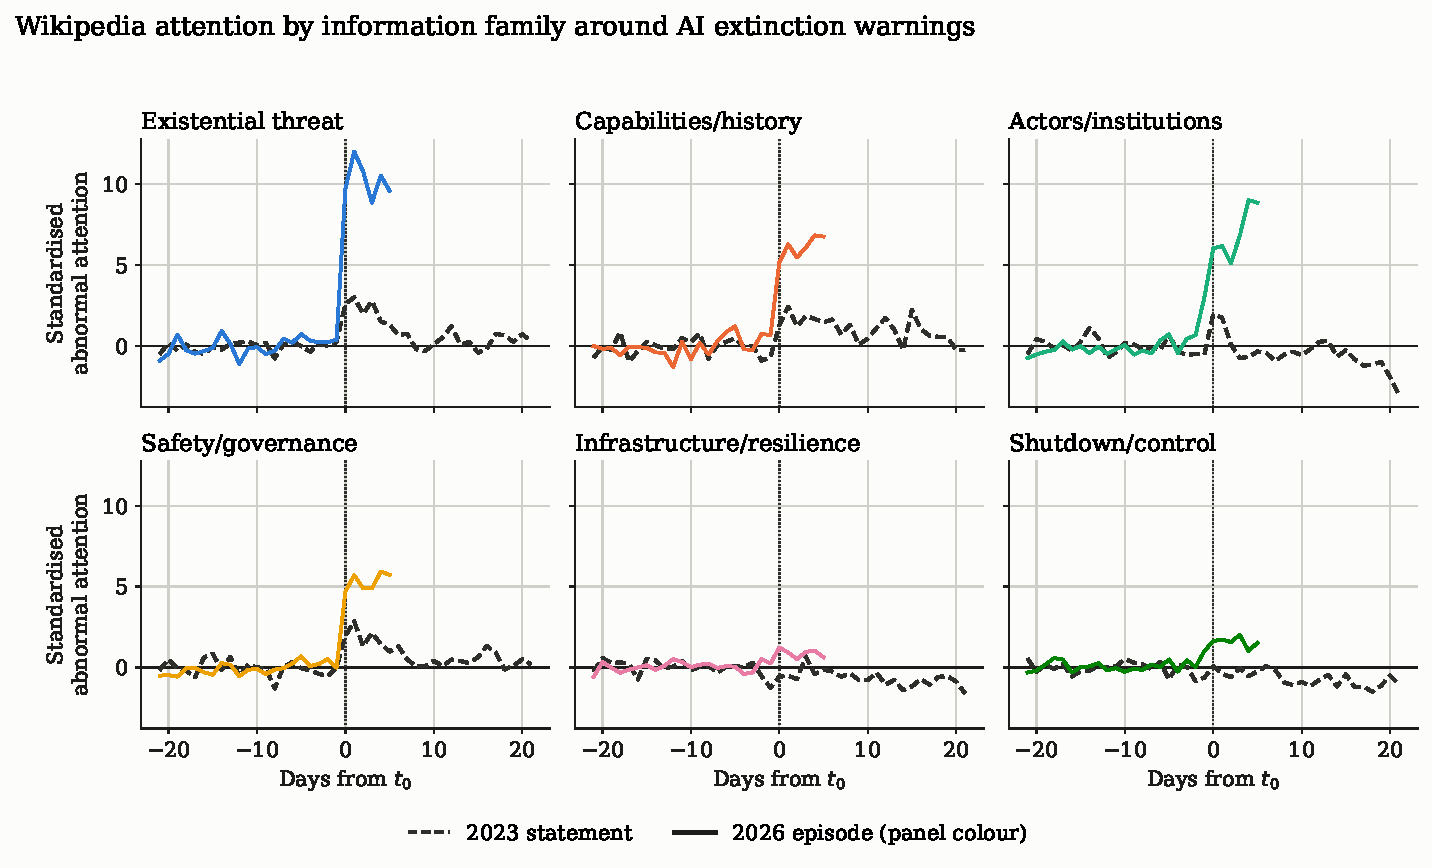
\includegraphics[width=0.98\linewidth]{figure_1_attention.pdf}
  \caption{\textbf{Standardized abnormal Wikipedia attention by information family.} Color identifies the family; the solid line is the September 2026 episode and the dashed gray line the May 2023 statement. Existential-threat attention rises by roughly an order of magnitude more than infrastructure attention and six times more than control attention. For 2026, the day before $t_0$ is scored out of sample, so the announcement-day rise in actor attention is visible. Both series are drawn only to $t_0+17$, the last day the pageviews API had published for the 2026 episode at the data cutoff; the 2023 window extends further but is truncated here so the two episodes are compared over an identical horizon.\label{fig:attention}}
\end{figure}

\begin{figure}[ht!]
  \centering
  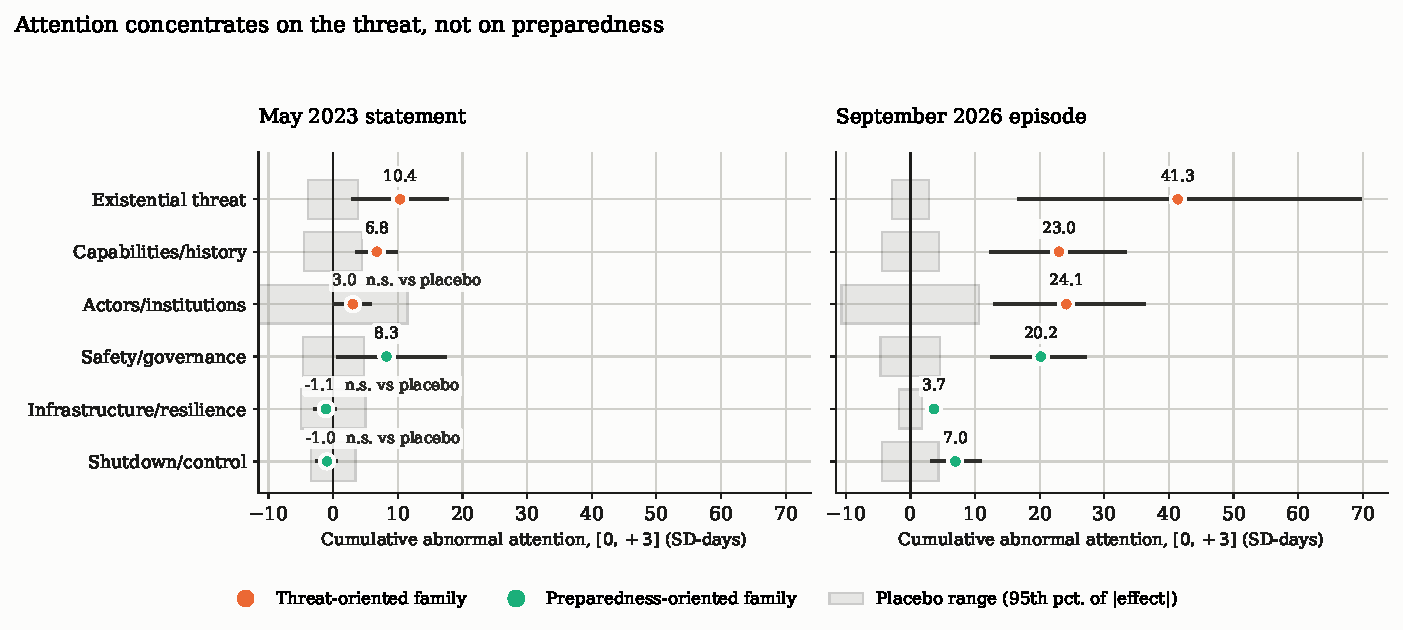
\includegraphics[width=0.8\linewidth]{figure_2_gap.pdf}
  \caption{\textbf{Attention concentrates far more on threat than preparedness.} Wikipedia page families, cumulative abnormal attention over $[0,+3]$ with bootstrap intervals. The gray band is the 95th percentile of $|$effect$|$ across placebo dates drawn from the same pre-event interval; an estimate inside the band is indistinguishable from background variation.\label{fig:gap}}
\end{figure}

In 2026, all six families exceeded their placebo ranges (\cref{fig:gap}), but the response was strongly concentrated on existential threat. Threat attention reached 41.3 SD-days, compared with 3.7 for infrastructure/resilience and 7.0 for shutdown/control---approximately 11 and 6 times larger, respectively. Actors/institutions (24.1), capabilities/history (23.0), and safety/governance (17.9) fell between these extremes.

\insightbox{Key finding.}{Existential-threat attention reached 41.3 SD-days in 2026, approximately 11x the infrastructure/resilience response and 6x the shutdown/control response.}

In 2023, only existential threat (14.0), safety and governance (8.3), and capabilities and history (6.8) exceeded their placebo ranges. Infrastructure and resilience ($-1.1$) and shutdown and control ($-1.0$) were indistinguishable from zero and slightly negative.

The longer prespecified windows, observable for both episodes at the 27 September 2026 cutoff, leave the central ratio intact. In 2026 the threat family cumulates to 75.2 SD-days over $[0,+7]$ and 101.8 over $[0,+14]$, against 6.0 and 9.8 for infrastructure/resilience and 13.1 and 20.7 for shutdown/control. The threat-to-infrastructure ratio is therefore 11.3, 12.5, and 10.4 across $[0,+3]$, $[0,+7]$, and $[0,+14]$: the imbalance is a stable feature of the episode rather than an artifact of where the window is cut. The mean daily threat--preparedness gap does decay as the episode ages, from 7.96 over $[0,+3]$ to 7.07 over $[0,+7]$ and 4.92 over $[0,+14]$, so the asymmetry narrows over two weeks without closing.

Two cautions attach to the longer windows, and both argue for keeping $[0,+3]$ as the primary result. First, negative-control drift grows with window length in 2023, from $-3.15$ over $[0,+3]$ to $-10.8$ over $[0,+7]$ and $-24.7$ over $[0,+14]$ (both $p<.001$), so the drift adjustment does progressively more of the work in the 2023 column and the adjusted long-window values should not be read as precise effects. Second, 2026 control drift, while never statistically distinguishable from zero, also grows ($+1.9$, $+5.5$, $+9.1$), and subtracting it leaves control-adjusted infrastructure/resilience attention at only 0.6 SD-days over both longer windows. The conservative reading is that infrastructure-oriented attention in 2026 is small and positive over $[0,+3]$ and not reliably distinguishable from background drift beyond it.

\Cref{tab:mainresults} reports both events side by side. Because negative-control pages reveal a baseline drift in the 2023 window (\cref{sec:robust}), the cross-event comparison uses drift-adjusted values.

\begin{table}[ht!]
\centering
\small
\caption{Cumulative abnormal attention over $[0,+3]$, in standardized
deviation-days, adjusted for negative-control drift}
\label{tab:mainresults}
\begin{threeparttable}
\begin{tabular}{lrrr}
\toprule
Information family & May 2023 & Sept. 2026 & Difference \\
\midrule
Existential threat & 17.1 & 39.5 & $+22.4$ \\
Capabilities/history & 9.9 & 21.1 & $+11.2$ \\
Actors/institutions & 6.2 & 22.3 & $+16.1$ \\
Safety/governance & 11.4 & 16.0 & $+4.6$ \\
Infrastructure/resilience & 2.0 & 1.8 & $-0.2$ \\
Shutdown/control & 2.2 & 5.1 & $+2.9$ \\
\midrule
Threat--preparedness gap (per day) & 2.97 & 7.96 & $+4.99$ \\
\bottomrule
\end{tabular}
\begin{tablenotes}[flushleft]\footnotesize
\item Drift adjustment subtracts the negative-control estimate for the same event and window ($-3.15$ for 2023, $p=.005$; $+1.86$ for 2026, $p=.30$). The 2026 adjustment is applied for consistency of rule, not because drift is detected; unadjusted 2026 values are 41.3, 23.0, 24.1, 17.9, 3.7, and 7.0, and the unadjusted 2023 values are 14.0, 6.8, 3.0, 8.3, $-1.1$, and $-1.0$. Unadjusted values and bootstrap intervals are in \texttt{outputs/tables/} and \texttt{data/derived/attention\_results.json}.
\end{tablenotes}
\end{threeparttable}
\end{table}


\subsection{The threat--preparedness gap (RQ3)}

The mean daily threat--preparedness gap \(TPG_e([0,+3])\) was 7.96 in 2026 and 2.97 in 2023, a 2.7-fold difference. Preparedness-oriented attention remained substantially lower than threat-oriented attention in both episodes.

\insightbox{Threat--preparedness gap.}{The mean daily threat--preparedness gap rose from 2.97 in 2023 to 7.96 in 2026, showing that threat-oriented attention grew much more than preparedness-oriented attention.}


\subsection{Media-frame and attention correspondence (RQ4)}
\label{sec:results-frames}

\Cref{fig:transmission} reports cumulative lag-0 to lag-3 associations between frame prevalence and matched family attention.

\begin{figure}[t]
  \centering
  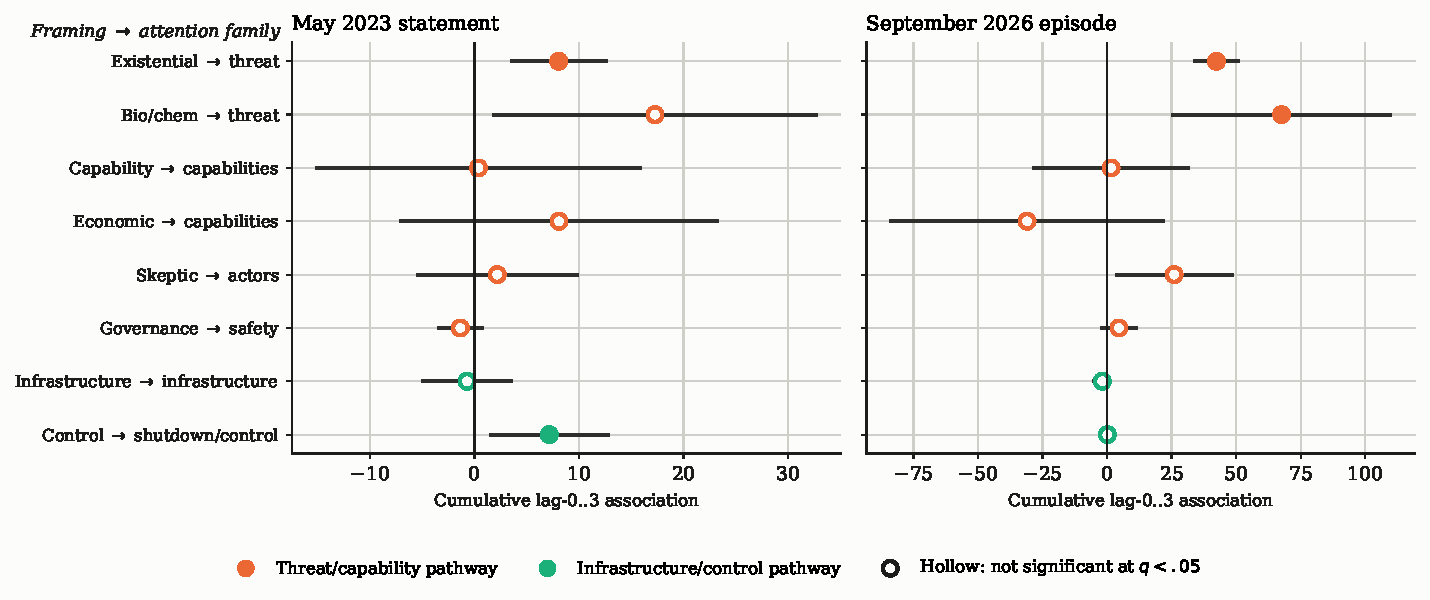
\includegraphics[width=0.98\linewidth]{figure_3_transmission.pdf}
\caption{\textbf{Existential media framing is associated with attention; infrastructure framing is not.} Cumulative same-day and lagged associations between media-frame prevalence and matched Wikipedia attention are shown for lags 0--3. Horizontal lines indicate 95\% confidence intervals, and filled markers survive Benjamini--Hochberg correction at $q<.05$. Existential framing is positively associated with existential-threat attention in both episodes, whereas infrastructure framing is not associated with infrastructure/resilience attention. Frame shares describe the targeted retrieved news corpus and should not be interpreted as population-level media prevalence. The panels use different horizontal scales.}
\label{fig:transmission}
\end{figure}

Existential framing was positively associated with existential-threat attention in both episodes (2026: 54.2, \(q<.001\); 2023: 10.9, \(q=.001\)). In contrast, infrastructure framing was not associated with infrastructure/resilience attention in either episode; the 2026 estimate is negative and does not survive correction (\(-2.6\), \(p=.050\), \(q=.057\)), and the 2023 estimate is indistinguishable from zero (\(-0.7\), \(p=.74\)). Biological/chemical framing also corresponded with threat attention in 2026 (54.0, \(q=.023\)), and control framing corresponded with shutdown/control attention in both episodes (2026: 1.6, \(q=.023\); 2023: 7.2, \(q=.049\)).

The 2026 panel is less selective than the 2023 panel: six of the eight prespecified pairs survive correction, including a large \emph{negative} association between economic framing and capabilities attention (\(-70.1\), \(q<.001\)) and positive associations for governance framing with safety attention (7.6, \(q<.001\)) and skeptic framing with actor attention (31.3, \(q=.023\)). We do not interpret the individual signs of these secondary pairs. The daily corpus is a ranked sample rather than a census, and re-drawing it changes day-level frame shares materially: collecting the same 2026 window twelve days apart moved shared-day frame shares by a mean absolute difference of .02--.04, which was enough to move four secondary pairs across the \(q<.05\) threshold while leaving the two theoretically matched pairs --- existential framing with threat attention, and infrastructure framing with infrastructure attention --- qualitatively unchanged in both direction and significance. The matched pairs are the claim; the secondary pairs are not stable enough at this corpus size to support one.

The null infrastructure correspondence is not evidence that infrastructure mechanisms were absent from the retrieved information environment. The corpus contained coverage of power-grid defense, OT security, cyberattack, infrastructure disruption, and related protective mechanisms. However, because mechanism-specific supplemental queries intentionally enriched the corpus for these topics, aggregate frame shares cannot be interpreted as estimates of their prevalence in the broader news environment or compared directly as measures of overall media emphasis. The narrower result is temporal: within the targeted retrieved corpus, day-to-day variation in the infrastructure-coded share did not correspond to day-to-day variation in infrastructure/resilience Wikipedia attention. These framing results remain provisional pending the human-validation procedure described in \cref{sec:scope}.

\insightbox{Cross-channel insight.}{Concrete infrastructure and protective mechanisms were present in the retrieved news stream, but infrastructure-oriented news content and infrastructure-oriented Wikipedia attention did not rise together.}


\subsection{Market divergence (RQ5)}

Over the 2026 episode (five trading sessions, 8--14 September), the cybersecurity/resilience portfolio produced a cumulative abnormal return of \(+11.3\%\) under the sector-adjusted market model. Its conventional 95\% interval excluded zero (8.7\% to 13.9\%), whereas the randomization-based result was marginal (\(p=.063\)). The corresponding estimates were \(-0.8\%\) for AI infrastructure and \(+3.5\%\) for AI platforms. The cybersecurity/resilience result was broad-based rather than driven by one security: ZS \(+14.6\%\), PANW \(+11.8\%\), CRWD \(+10.6\%\), and FTNT \(+8.2\%\). It retained the same sign under the broad-market specification and after excluding the security flagged for a firm-specific announcement (\(+10.2\%\)).

The three prespecified post-event windows, which required sessions that had not yet traded at the earlier data cutoff, are now complete and reproduce this ordering (\cref{fig:market}). The cybersecurity/resilience estimate is \(+12.9\%\) over \([-1,+1]\) (\(p=.014\)), \(+13.6\%\) over \([-3,+3]\) (\(p=.063\)), and \(+13.0\%\) over \([0,+5]\) (\(p=.052\); \(+14.3\%\), \(p=.029\), under the broad-market specification). Across the same windows AI infrastructure ranges from \(-1.6\%\) to \(+1.3\%\) and AI platforms from \(+3.0\%\) to \(+3.9\%\), neither reaching conventional significance. Excluding flagged securities --- ZS in every window, and META in \([0,+5]\) --- reduces the cybersecurity/resilience estimate to between \(+9.6\%\) and \(+11.0\%\) without changing its sign or its rank among the three portfolios. \Cref{fig:divergence} places this ordering beside the attention result: within the equity channel resilience providers are repriced the most, while within the public-attention channel the resilience families are the smallest responses. Abnormal trading volume for that portfolio remained near normal throughout, ranging from \(-0.10\) to \(+0.24\) in log points across the four windows.

\begin{figure}[ht!]
  \centering
  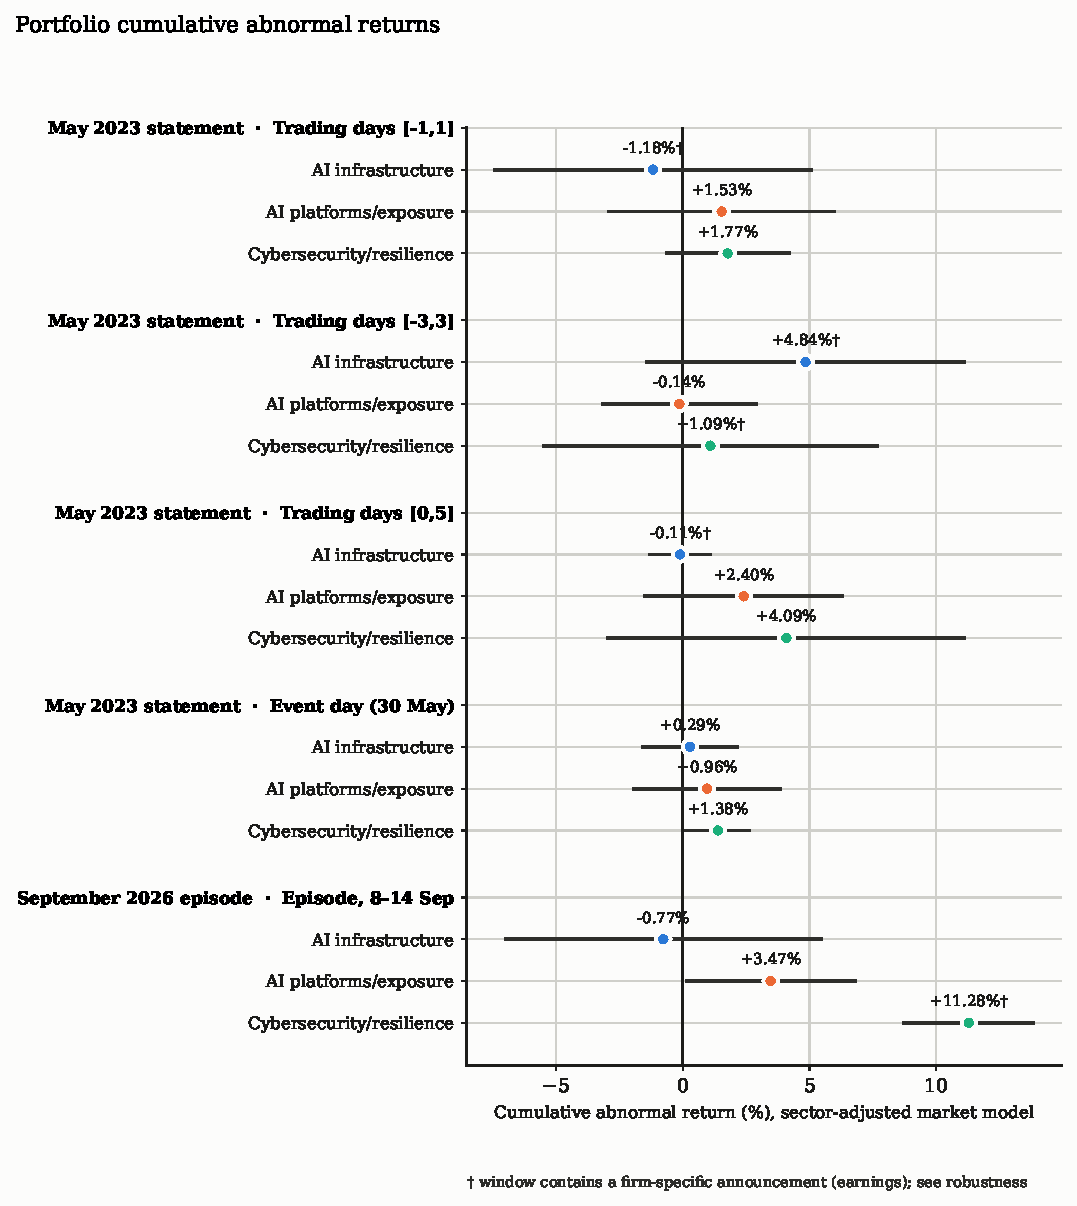
\includegraphics[width=0.89\linewidth]{figure_4_market_car.pdf}
\caption{\textbf{Cybersecurity and resilience firm stocks outperformed during the 2026 AI warning episode.} Portfolio cumulative abnormal returns are shown with 95\% confidence intervals under the sector-adjusted market model. Positive values indicate performance above the modeled benchmark. The 2023 AI-infrastructure estimate over $[-3,+3]$ is confounded by earnings releases and is not interpreted as an event response.}
\label{fig:market}
\end{figure}


\begin{figure}[ht!]
  \centering
  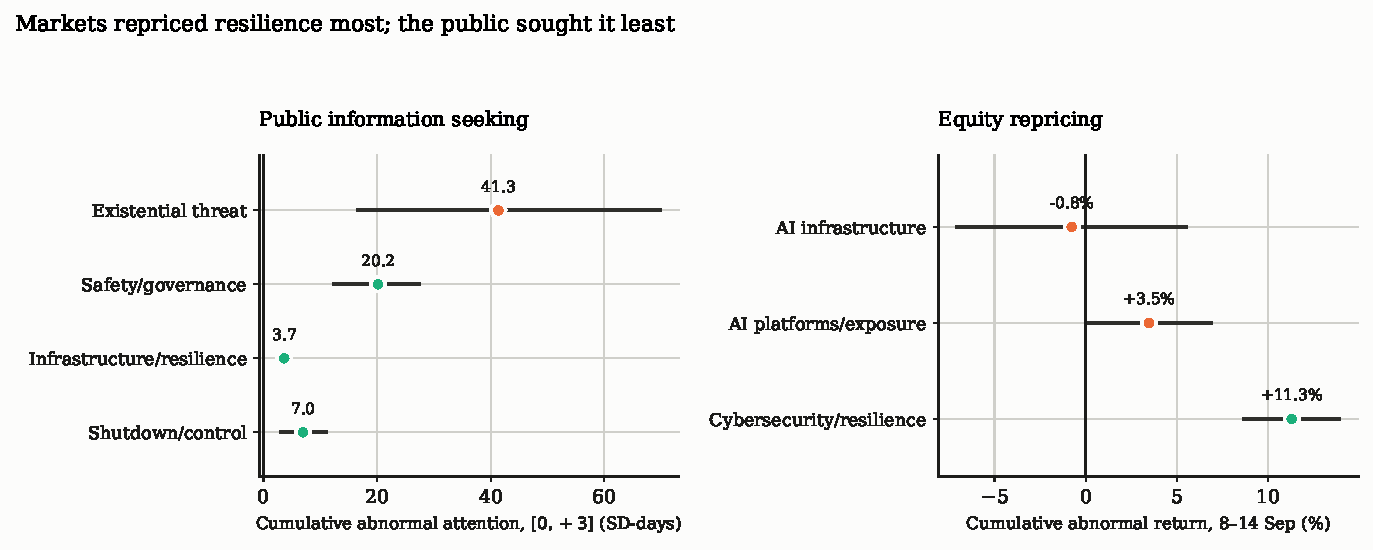
\includegraphics[width=0.98\linewidth]{figure_5_divergence.pdf}
\caption{\textbf{The channel that repriced resilience most is the one the public sought least.} Left: cumulative abnormal Wikipedia attention over $[0,+3]$ for the threat family and the three preparedness families, with bootstrap intervals. Right: portfolio cumulative abnormal returns over the 8--14 September episode, with 95\% intervals. The two panels measure different quantities --- standardized attention and percentage abnormal return --- and are deliberately not drawn on a common axis; the comparison they support is the ordering within each channel, not a numerical equivalence between them.}
\label{fig:divergence}
\end{figure}

\insightbox{Cross-channel divergence.}{Public information seeking concentrated on catastrophic AI risk, while the largest equity-market response occurred among cybersecurity/resilience firms (\(+11.3\%\) cumulative abnormal return).}


\subsection{Robustness and falsification}
\label{sec:robust}

\paragraph{Negative controls and baseline drift} Negative controls showed no detectable drift in 2026 (\(+1.86\), \(p=.30\)) but a negative shift in 2023 (\(-3.15\), \(p=.005\)), reflecting late-May seasonality in several control pages. Cross-event comparisons therefore use estimates adjusted for the corresponding control-page drift (\cref{tab:mainresults}).

\paragraph{Placebo dates} Twelve placebo dates per event were drawn deterministically from the pre-event interval with a seven-day exclusion zone around $t_0$ and around the known kill-switch policy dates, and each is modeled with the same baseline design as the true event (56 days, with the same gap before the pseudo-event). Results appear as the gray band in \cref{fig:gap}. Every 2026 family clears its band; shutdown and control do so by the smallest margin among the families that respond (7.0 against a 95th percentile of 4.3), and its leave-one-page-out range (5.6 to 8.1) stays above the band.

\paragraph{Specification and composition} The main ordering is robust to alternative baseline lengths, shifting the 2026 event date to 8 September, excluding event-named pages, leave-one-page-out tests, and cumulating over $[+1,+3]$ instead of $[0,+3]$. The largest sensitivity concerns actors/institutions: treating 8 September as part of the baseline reduces that estimate from 24.1 to 11.2 because several actor pages had already risen sharply that day. Infrastructure/resilience remains between 3.4 and 4.0 SD-days and shutdown/control between 5.6 and 8.1 across leave-one-page-out tests. A local-level structural time-series counterfactual also reproduces the overall pattern \citep{brodersen2015causalimpact}.

\paragraph{Platform-wide traffic} Normalizing family views by total English Wikipedia user traffic gives post/pre share ratios of 7.17 for existential threat against 1.10 for infrastructure and 1.65 for control in 2026, confirming that the result is topic-specific rather than a platform-wide change.

\paragraph{The kill-switch series} Removing the broad \emph{Kill switch} article from the control family \emph{raises} the 2026 estimate slightly (6.96 to 7.47), so the family result is not produced by that single page. The article itself shows a cumulative effect of 3.4 SD-days, within placebo range.

\paragraph{Firm-specific announcements} A security is flagged when it shows both heavily elevated volume and a large abnormal return inside an event window. This check overturns one result: the only conventionally significant 2023 portfolio estimate --- AI infrastructure $CAR[-3,+3]=+4.84\%$, randomization $p\approx 0$ --- is driven by NVDA ($+10.5\%$) and AVGO ($+9.4\%$), both of which reported earnings inside that window. Excluding flagged securities leaves $-0.30\%$. Therefore, we do not interpret any 2023 market estimate as a response to the Statement on AI Risk.


\subsection{Scope of the analysis}
\label{sec:scope}

\paragraph{2023 event-named pages} \emph{Statement on AI Risk}, \emph{Pause Giant AI Experiments}, \emph{Dario Amodei}, and \emph{Existential risk studies} had no pre-event baseline in May 2023 (an article created by the event cannot have a counterfactual) and were removed under the ``insufficient baseline observations'' rule. The safety and governance family therefore rests on four pages in 2023 against seven in 2026, which is one reason the cross-event comparison is reported with drift adjustment and family sizes stated.

\paragraph{Frame validation is not complete} The frame indicators used in \cref{sec:results-frames} are automated keyword-dictionary labels applied to headlines only. The preregistered procedure requires a further step that has not yet been carried out: two independent coders label a stratified sample of the retrieved corpus, intercoder reliability is computed as Krippendorff's \(\alpha\) \citep{krippendorff2018content}, and a frame is admitted to the substantive analysis only if the automated labels reach a macro-F1 threshold against the human labels. The stratified 400-item sample is exported by the pipeline (\texttt{data/derived/frame\_coding\_sample.csv}) with blank coder columns and the automated label retained for comparison; the reliability fields in the run manifest remain null until it is coded. \textbf{All frame-based results (RQ4) are therefore provisional.} The sentiment measures reported alongside the frames use VADER \citep{hutto2014vader} as a transparent lexical baseline and are subject to the same caveat.

\paragraph{Window coverage} At the 27 September 2026 cutoff all three prespecified attention windows and all three prespecified market windows are observed for both episodes, so no result in this paper is reported on a partially observed window. The 2026 Wikipedia observation window nominally extends to $t_0+28$ (7 October 2026); days beyond the API publication cutoff of 26 September are recorded as unobserved rather than zero and enter no estimate.


\section{Discussion}

\subsection{Threat attention dominates infrastructure-oriented attention}

The central finding is an imbalance, not an absence, of preparedness-oriented attention. Infrastructure/resilience attention increased in 2026, but the existential-threat response was approximately eleven times larger. In 2023, infrastructure/resilience and shutdown/control did not exceed background variation. Together, the episodes show that heightened attention to catastrophic AI risk does not translate proportionally into attention to protective capacity.

The framing analysis reinforces this distinction. Infrastructure mechanisms were present in the news corpus, but day-to-day infrastructure framing did not correspond with infrastructure/resilience Wikipedia attention; existential framing did correspond with threat attention. Because the retrieval strategy enriched specific topics, this result concerns temporal correspondence rather than broader media prevalence.


\subsection{Two populations, two responses}

The equity-market channel showed a different ordering. During the 2026 episode, cybersecurity/resilience firms produced the largest portfolio abnormal return while infrastructure/resilience remained the smallest Wikipedia-family response. The pattern is now visible in all four market windows rather than only the episode window, and it survives excluding the securities flagged for firm-specific announcements, which strengthens it relative to the earlier partial-window result. The interpretation nonetheless remains tentative: investor motives are unobserved, the portfolio holds only four securities, randomization evidence is significant in some windows ($p=.014$ over $[-1,+1]$) and marginal in others ($p=.063$ over the episode and $[-3,+3]$), and trading volume was not unusually high in any of them. The defensible conclusion is therefore that the two aggregate channels displayed different relative emphases.


\subsection{Implications for infrastructure risk communication}

If warnings increase threat salience much more strongly than attention to protective capacity, communicators may be telling audiences \textit{what to fear} without providing an equally salient path toward response. This interpretation is consistent with theories that distinguish threat appraisal from efficacy and protective action \citep{witte1992eppm,kahlor2010prism}. The implication is not that existential risk warnings should be suppressed. Rather, their protective content was reflected much less strongly than their threat content in the Wikipedia behavior observed here.

We offer three practical observations. First, infrastructure-related coverage did not correspond with greater infrastructure-oriented Wikipedia attention. Second, safety/governance attracted substantially more attention than infrastructure/resilience or shutdown/control, suggesting stronger interest in institutional mitigation than operational protection. Third, Wikipedia behavior should not be interpreted as infrastructure-operator readiness; that question requires operator-facing evidence such as advisory use, exercises, continuity planning, and incident-response activity.

\insightbox{Practical insight.}{Making protective information available may not be sufficient to redirect attention toward preparedness: concrete infrastructure, cybersecurity, control, and governance mechanisms were present during the episode, yet threat-oriented attention remained dominant.}


\subsection{Why the attention gap matters}

Information seeking matters because it provides an observable indication of what aspects of a risk people are trying to understand. Prior studies of public health crises show that online information seeking responds strongly to news exposure and can provide a behavioral trace of collective awareness and response \citep{tizzoni2020zika,gozzi2020covid}. Risk communication research also emphasizes that communicating a threat is not sufficient; audiences need information about efficacy and possible responses if heightened concern is to support action \citep{witte1992eppm,schwarz2024rage}.

In this study, the threat--preparedness gap matters because it captures whether heightened attention to catastrophic AI risk is accompanied by attention to ways of managing that risk. A large positive TPG does not show that individuals are unprepared or will fail to act. Rather, it indicates that the observable information-seeking response is weighted more toward catastrophic consequences than toward safety, infrastructure resilience, and control mechanisms. For critical infrastructure protection, this distinction is consequential: making a threat salient is not the same as making protective capacity salient.


\subsection{Limitations}

This study has several limitations. 
Wikipedia pageviews are aggregate behavioral traces, not unique users, beliefs, emotions, or evidence of preparedness; English Wikipedia is also not representative of the public or of infrastructure operators. Temporal correspondence among news, Wikipedia attention, and markets does not establish causality. The 2026 episode also overlaps with other policy, corporate, and macroeconomic developments. Granger-causality testing was not appropriate because the short event windows provide too few daily observations for reliable lagged time-series inference. 
The deterministic frame classifier removes case-by-case coder discretion but does not eliminate measurement error or researcher judgment: keyword choices define the operationalization, and lexical matching may miss context, ambiguity, negation, or language not represented in the dictionary. Accordingly, frame results concern the prevalence of the specified framing language rather than a complete semantic interpretation of news coverage.
Finally, page-family definitions involve judgment, and Wikipedia traffic can change because of article creation, renaming, or prominent linking rather than underlying information demand.


\subsection{Future work}

Future work should compare additional Wikipedia language editions, and use surveys or operator-facing data to measure protective intentions and readiness directly.


\section{Conclusion}

AI extinction warnings are communication events as well as claims about technological risk. Across two prominent episodes, the warnings were followed by much greater attention to catastrophic consequences than to infrastructure resilience or emergency control. The distinction was one of magnitude, not complete absence: infrastructure/resilience attention
exceeded its placebo range in 2026, but the existential-threat response was approximately eleven times larger.

The equity-market channel displayed a different ordering. Cybersecurity/resilience firms produced the largest portfolio abnormal return in every prespecified 2026 window, although randomization-based evidence was significant in some windows and only marginal in others, and abnormal trading volume did not increase. For critical infrastructure protection, the practical implication is that heightened salience of catastrophic AI risk should not be interpreted as a proportional orientation toward protection. Measuring threat attention, preparedness-oriented attention, and market repricing separately reveals a response profile that any single channel would miss.

For critical infrastructure protection, the broader implication is that successful risk communication should not be evaluated solely by whether a warning attracts attention. It also matters where that attention goes: making a threat salient is not the same as making protective capacity salient.


\section*{Ethics and Data Governance}

The study uses aggregate public pageview counts, public news metadata, and market data. It does not attempt to identify individual Wikipedia users or infer sensitive individual attributes. The final manuscript will report the relevant institutional determination concerning human-subjects review. Copyrighted news text is not redistributed; derived labels, URLs, queries, code, and aggregate results are shared.

We carried out data collection, analysis, and figure generation in Python 3.12.1. We retrieved data using the Python standard library (urllib) from the Wikimedia REST Pageviews API, MediaWiki API, Google News RSS, and Financial Modeling Prep. We used NumPy 2.5.1 and pandas 3.0.3 for data handling. We estimated attention models with statsmodels 0.15.0, using SciPy 1.18.1 for distributional tests. Figures were rendered with Matplotlib 3.11.0.

Declaration of generative AI use. During the preparation of this work, the author(s) used Claude (Anthropic) to help write and debug the data-collection code, and to generate figures. After using this tool, the author(s) reviewed all code and take full responsibility for the publication's content.


\section*{Data and Code Availability}

Analysis code, configuration files, page-family definitions, event dates, and derived outputs are available in the supplementary material zip folder. The pipeline writes a machine-readable manifest containing package versions, run timestamps, random seeds, per-ticker data source, and SHA-256 hashes of each configuration file. Market data requires a Financial Modeling Prep API key supplied through the environment; no key is stored in the supplementary materials.

\section*{Disclaimer}
\textit{The views expressed are those of the authors and do not necessarily reflect the official policy or position of the United States Air Force, the Department of Defense, or the U.S. Government.
}
\ifelsevierclass
  \bibliographystyle{elsarticle-num}
\else
  \bibliographystyle{unsrtnat}
\fi
\bibliography{references}

\scriptsize
\begin{center}

\begin{longtable}{
>{\raggedright\arraybackslash}p{0.17\textwidth}
>{\raggedright\arraybackslash}p{0.75\textwidth}}

\caption{\scriptsize Complete lexical dictionary used for automated news-frame classification}
\label{tab:framedictionary}\\

\toprule
Frame & Words and phrases used for classification \\
\midrule
\endfirsthead

\multicolumn{2}{c}{\scriptsize\textit{Table \thetable\ continued}}\\
\toprule
Frame & Words and phrases used for classification \\
\midrule
\endhead

\bottomrule
\endfoot

\textbf{Existential threat} &
extinction;
existential;
end of humanity;
wipe out humans;
kill us all;
kill all humans;
kill humanity;
human survival;
doom;
loss of control;
out of control;
rogue AI;
takeover;
annihilation / annihilate;
catastrophe / catastrophic;
apocalypse / apocalyptic;
threat to humanity
\\[0.5em]

\textbf{Infrastructure} &
critical infrastructure;
power grid;
grid;
pipeline;
water system;
cyberattack / cyber attack;
cybersecurity / cyber security;
hacking;
ransomware;
blackout;
cascading failure;
supply chain;
telecommunications / telecom;
data center / data centre;
utility / utilities
\\[0.5em]

\textbf{Biological/ chemical} &
biological weapon;
bioweapon;
biosecurity;
pathogen;
chemical weapon;
pandemic;
virus design;
bioterror / bioterrorism
\\[0.5em]

\textbf{Economic disruption} &
job / jobs;
unemployment;
labor market / labour market;
workforce;
layoff / layoffs;
wage / wages;
economic disruption;
automate / automation / automating;
displaced worker / displaced workers;
worker displacement;
bubble;
market rout;
market selloff;
market plunge
\\[0.5em]

\textbf{Governance} &
regulation / regulate / regulatory;
legislation / legislative;
bill;
law;
Congress;
lawmaker / lawmakers;
Senate / senator;
policy / policymaker;
governance;
oversight;
moratorium;
pause;
slow down / slowdown;
ban;
treaty;
White House;
EU AI Act;
safety institute;
accountability / accountable
\\[0.5em]

\textbf{Control} &
kill switch / killswitch;
emergency shutdown;
shut down / shut it down;
off switch;
fail-safe / failsafe;
containment;
interruptibility / interruptible;
circuit breaker;
capability control;
guardrail / guardrails
\\[0.5em]

\textbf{Capability} &
superintelligence;
AGI;
artificial general intelligence;
self-improvement / self-improving;
recursive / recursive self-improvement;
frontier model;
scaling;
breakthrough;
more powerful;
capability / capabilities;
autonomous agent;
reasoning model
\\[0.5em]

\textbf{Skepticism} &
hype;
overblown;
skeptic / skeptical;
sceptic / sceptical;
dismiss / dismisses / dismissed;
nonsense;
fearmongering / fear mongering;
doomer;
hysteria / hysterical;
distraction;
overstated / overstatement;
rejects warning / reject warning;
pushes back / push back
\\

\end{longtable}

\vspace{-0.5em}

\begin{minipage}{0.92\textwidth}
\scriptsize
\textit{Note.} Entries are shown in human-readable form for transparency. The classifier uses case-insensitive lexical matching, including spelling and morphological variants represented here with slashes. Classification is nonexclusive, so a headline may receive more than one frame label. The exact machine-readable regular expressions used in the analysis are provided in the supplementary source code.
\end{minipage}

\end{center}


\begin{table}[ht!]
\centering
\small
\caption{Representative headline matches produced by the automated frame classifier}
\label{tab:frameexamples}

\begin{tabular}{
>{\raggedright\arraybackslash}p{0.16\linewidth}
>{\raggedright\arraybackslash}p{0.55\linewidth}
>{\raggedright\arraybackslash}p{0.20\linewidth}}
\toprule
Frame & Representative retrieved headline & Triggering pattern \\
\midrule

Existential threat &
\emph{AI could pose `existential' risk to humanity, UN rights chief warns}
(Reuters, 2026) &
\texttt{existential} \\

Infrastructure &
\emph{Chinese supply chains for critical infrastructure threaten the US power grid}
(Utility Dive, 2023) &
\texttt{critical infrastructure};
\texttt{power grid};
\texttt{supply chain} \\

Biological/ chemical &
\emph{`All it will take is one screw-up': AI groups race to limit bioweapon risks}
(Financial Times, 2026) &
\texttt{bioweapon} \\

Economic disruption &
\emph{AI: Which jobs are most at risk from the technology?}
(BBC, 2023) &
\texttt{jobs} \\

Governance &
\emph{Governments race to regulate AI tools}
(Reuters, 2023) &
\texttt{regulat} \\

Control &
\emph{Lords call for AI `kill switch' powers in UK}
(BBC, 2026) &
\texttt{kill switch} \\

Capability &
\emph{AI `more powerful by the day', Anthropic co-founder tells BBC}
(BBC, 2026) &
\texttt{more powerful} \\

Skepticism &
\emph{Charlie Munger is skeptical of AI: `Old-fashioned intelligence works pretty well'}
(CNBC, 2023) &
\texttt{skeptic} \\

\bottomrule
\end{tabular}

\begin{minipage}{0.94\linewidth}
\footnotesize
\textit{Note.} Examples are drawn from the retrieved corpus and are shown only
to illustrate the deterministic lexical matching procedure. They are not
manually selected reference labels or evidence of classifier accuracy. Frames
are nonexclusive; a headline may satisfy more than one dictionary.
\end{minipage}
\end{table}

\end{document}